\documentclass[a4paper, 12pt]{article}

\usepackage{draftwatermark}
\usepackage{changepage}
%\usepackage{fullpage}
\usepackage{color}
\usepackage{xcolor}
\usepackage{listings}
\usepackage{array}
\usepackage{multirow}
\usepackage{footnote}
\usepackage{graphicx}
\usepackage{verbatim}

\SetWatermarkScale{4}
\SetWatermarkText{}
\SetWatermarkLightness{0.9}

\usepackage{caption}
\DeclareCaptionFont{white}{\color{white}}
\DeclareCaptionFormat{listing}{\colorbox{gray}{\parbox{\textwidth}{#1#2#3}}}
\captionsetup[lstlisting]{format=listing,labelfont=white,textfont=white}
\lstset{
	tabsize=4,
	basicstyle=\footnotesize,
	columns=fixed,
}

\parindent0pt
\parskip10pt
\makesavenoteenv{tabular}

\title{Self-Describing Bus (SDB) Specification\\
for Logic Cores -- proposed Version 1.1}
\author{Alessandro Rubini (Consultant for CERN)\\
Wesley Terpstra (GSI),\\
Manohar Vanga (CERN, BE/CO/HT)}
\date{March 28th 2013}
\begin{document}

\maketitle

\tableofcontents
\listoftables
%\listoffigures

\pagebreak

\section*{Bugs}

Even though the project already passed the 1.0 milestone, there are still some
things that ought to be changed or added:

\begin{itemize}
\item We should clarify that  addresses in nested buses are relative to the sub-bus;
\item The description of the record type should get a more prominent place than the
  current description in the \textit{product} structure;
\item We need a policy for designers adding class etc, and it must be described;
\item A reference implementation exists, but it is not described here.
\end{itemize}

\section*{Versioning}

The SDB specification is the work of people discussing in the
\texttt{fpga-config-space} mailing list, using the IETF approach of
``rough consensus and running code''. Everybody can join and contribute.

The mailing list is part of the project
with the same name on \texttt{ohwr.org}. The direct
link is \texttt{http://www.ohwr.org/projects/fpga-config-space} .

This document describes a post-1.0 (But pre-1.1) status. It describes version 1 of the data
structures. All future \textbf{compatible} releases of this
specification will be blessed 1.\textit{x}, for some ever-increasing
version of \textit{x}.  A compatible specification is one that
explains better some unclear points (see ``Bugs'' above) or that adds
record types that may be identified (and possibly ignored) by previous
parsers.

If we ever need to release version 2 (or further) of the SDB
structures, the specification version will be raised accordingly. New
specifications will continue to describe older versions of the data
structures, and parsers running on host computers will be required to
still parse the older versions.  (No such requirement is there for
soft-cores, because the parser code is synthesized together with the data
structures).

\section{Introduction}

This document describes a specification for a series of self description
structures that can be used to provide metadata about logic blocks. This metadata
should be provided by the logic cores, like PCI or USB description records do,
so device drivers and other software can automatically discover the blocks and
configure them at runtime.

\subsection{History and Rationale}

The idea of a self-description for a  bus appeared while working on
\textit{White Rabbit} and related projects that make massive use of
FPGA devices. Separately and concurrently, both the CERN and the GSI
working groups identified the need for some way to self-detect the
contents of a specific logic device after it is programmed.

We envisioned that if the internal FPGA bus could enumerate its own
content, we would get the following advantages:

\begin{itemize}
\item Run-time validation of FPGA binary images;
\item Easy matching of software and gateware;
\item Automatic handling of several binaries with the same software;
\item Feasibility of tools similar to \texttt{lspci} and \texttt{lsusb};
\item Automatic loading of kernel drivers on the host computer;
\item Automatic setup of low-level drivers within soft cores;
\item Better decoupling of gateware and software development.
\end{itemize}

As usual in engineering, we wanted a system that was as simple as possible,
yet open to future extensions without introducing compatibility issues.
While our internal bus is \textit{Wishbone}, we designed the structures
to be generic so other bus implementations may use them. 

We are aware of the AMBA (PrimeCell) cell-id standard, but we think it
is seriously under-designed: the idea is sound, but a single cell-ID field
is not enough if we want to make sense of the whole bus. We think current
hardware and software resources allow a richer description of logic blocks.

We are also aware of the PCI and USB data structures, but they are
unsuitable for an FPGA, either. First of all, they assume devices are
enumerated by other means whereas we need to be able to scan a flat
address space; then, their vendor ID space is not wide enough to allow
small developers to easily participate.

This specification, thus, uses 64 bits for the vendor ID, to prevent scarcity.
The vendor space is split in two parts, and all users are free to bless their
own vendor number and start designing using these data structures,
provided the most-significant vendor-id bit is set.

We acknowledge the usefulness of a central vendor registry, so
the lower half of the
vendor-ID space is reserved for numbers that
are officially assigned and published.  The vendor registry, however, is not
part of this specification, which just lists the first few vendor-ID values that
have already been used.

All multi-byte values are stored in \textit{big endian} order.  We need
a well-defined endianness to allow generic scanning of the target bus;
we picked big-endian because most embedded devices are big endian and
because  it is the format usually chosen by existing standards documents.

All data structures are 64 byte in size and they are all similar in their
internal layout; the last byte in the 64-byte slot identifies the type
of each structure, to allow very simple parsing code and easy extension
to new types of structures.  The size is a power of two in order to
avoid multiplication and division in calculation of sizes, as the
driver may reside in a very simple soft-core.


\subsection{Scope of This Specification}

This specification documents the format used by CERN and GSI. However,
everyone is welcome to use the data structures defined in this
specification (or customized derivatives) in their own work.

Parts of this document are written in the language of
a formal specification because we need clear and sharp rules in
order to make different implementations interoperate.  We are sticking
to those rules in our own implementations, both in gateware and in
associated software.

Everybody is free to choose a vendor-ID and start coding right now; we
suggest to pick a random 64 bit number and set the most significant
bit (as an alternative, you can paste the bit ``1'' in front of
a random 63 bit number).

If you want to implement your own self-description ROM, because you like
this idea but want to do it differently, please change the magic number, so to avoid
headaches if both bus implementation are instantiated within the same host
computer or network.


\subsection{Interrupts}

This version of SDB doesn't describe interrupts.  Lack of interrupt
description is a design choice.

SDB was born as a description of address spaces. Access to address
spaces is usually done through \textit{bus} signals, according to the
bus specification: signal lines, protocols, timings.  Interrupts
strictly-speaking are not part of the bus: they are a sort of a
``secondary'' bus, where only one signal line connects one core to the
``interrupt controller'' core.  The same applies to the out-of-band
DMA channels used in some designs, where two devices are connected via
a path not part of the normal bus interconnect fabric.

Neither of these is strictly in the scope of SDB; but especially as
far as interrupts are concerned, we really think FPGA designs should
be converted to the concept of MSI interrupts. Message-signalled
interrupts have a number of advantages over legacy interrupts, and
don't even need any description besides what SDB already offers.

A more complete discussion of this is in the wiki page of the project:

\texttt{http://www.ohwr.org/projects/fpga-config-space/wiki}.

On the other hand, it may make sense to define SDB structures to
describe this special wiring, when it exists, to help existing
``legacy'' projects to benefit from SDB and avoid doping the software
source code with static information about device wiring.  Thus,
it may happen that future
releases of this specification include description of legacy
interrupts.

\subsection{The Overall System Structure}

The bus described by the structures defined herein is set up as a
flat address space. Our initial target is the \textit{Wishbone} bus,
as used in our own FPGA projects, but the overall situation is
pretty general and can be applied to any bus or even a storage
system for quasi-static information in flash memory

To keep variety to a minimum, this standard defines the concept of
\textit{product}, which is anything that has been \textit{done}, and thus has
its own identifiers, name, version and date.  This includes some of
the meta-information structures, for example a record of the final build of the
FPGA binary.

Every \textit{product} that lives in some address range is called a
\textit{component}; as such it specifies its first and last address, both as
64 bit numbers.

Within the bus memory area, the address space available to bus masters
is usually decoded into several blocks using the high address bits, so
that the space is divided into address areas. Usually the areas are sized
as powers of two, but this is not mandatory -- some designers may use
individual address lines to select blocks, to easily get a sparsely
populated address space.  The designer of the address demultiplexer
(the \textit{interconnect} block) is expected to describe the
logic blocks living behind the interconnect, as well as the
interconnect itself. Thus, the \textit{interconnect} is a \textit{component}
(so that it owns an address range), and the associated SDB record is the first
one of an array of structures; the other records on the array
defines the \textit{components} that are connected downstream of this multiplexer
and optionally more abstract \textit{products}.

Some of the blocks within the data space of an \textit{interconnect}
component can in turn be
bridges to other \textit{interconnect} components.  Thus, the \textit{bridge}
component states the address where further self-description structures are to
be found. This allows nesting at arbitrary levels (too deep nesting is
not a good practice, but this specification is not limiting the
designer's ingenuity).

Only the bus designer knows where the outer-level data structure is to
be found, and such information is expected to be known by the ``bus
driver'' software package.  For example, a soft-core scanning its own
bus will know where to start from, because it is part of the same
overall design; a PCI driver must know how to access internal bus
memory from a PCI memory window, so it can also know where the
SDB entry point is stored; an \textit{Etherbone} bus master will
comply to its own packet-format standard, so it can as well know
where to start enumerating the remote bus from.

We can therefore define a number of terms to build the
self-description framework. What follows is the list of data
structures and sub-structures defined by SDB. Each
structure represents a specific abstraction: the name of the
structure matches the SDB definition of the respective term:

\begin{description}
\item[Product] \hfill \\
Every structure includes \textit{product} fields, i.e.
the vendor and device identifiers, version and date, and an UTF-8
name.

\item[Component] \hfill \\
A component is a \textit{product} with an associated address range. Its
structure lists the first and last valid addresses within
the encompassing address space and includes a \textit{product}
structure. The addresses are relative to the hosting \textit{interconnect}.

\item[Interconnect] \hfill \\
The \textit{interconnect} is a \textit{component} representing an address demultiplexer.
The associated data structure is the first in an array of \textit{product} descriptions;
its specific fields are magic number, bus type, version and the number of
structures in the array.

\item[Device] \hfill \\
The \textit{device} component identifies a peripheral block, with
its class, ABI version and bus-specific flags.

\item[Bridge] \hfill \\
The \textit{bridge} component marks a memory area leading to a lower-level
address demultiplexer (i.e. an \textit{interconnect}). Its data
structure declares the address where the self-description for the
sub-bus is to be found, relative to the hosting \textit{interconnect}.

\item[Integration] \hfill \\
The optional \textit{integration} product describes an aggregate bus.
It is a \textit{product} record, not a
\textit{component}, in that it has no associated address range. This
meta-information item can be used by a vendor to describe
its particular combination of devices, interconnect, and address layout.
For example, if an expansion card uses a number of stock devices
combined with a stock interconnect, its driver can nonetheless recognize
the aggregate device by the integration record.

\end{description}

The other term we need to to define is \textit{controller},
which is listed separately because it doesn't match any data structure:

\begin{description}
\item[Controller] \hfill \\
The \textit{controller} is a software abstraction, used in the host
computer driving the bus (if any). The controller defines the
methods to access its own bus and knows where the outer SDB
array is found.  There is no controller concept for soft-cores
that  self-scan their own address space.

\end{description}

\subsection{Current Implementations}

The self-description mechanisms described here are already
successfully used by the Etherbone project, whereas FPGA devices
equipped with an Ethernet port allow external hosts to be bus masters
in the internal Wishbone bus.  The host computer can completely
describe and access the remote bus(es) using the structures described
here; by identifying each instantiated device it can also drive the
remote peripherals without prior knowledge of the specific FPGA binary
it is talking to.

The same mechanism is already part of the \textit{White
Rabbit PTP Core} and the outer-level FPGA designs that are
being used in our synchronized I/O boards.


\section{SDB Header Material}

This section includes the whole header file that defines the data
structures. The header itself is included in the source code
that accompanies this specification.

All fields and bits are explained in detail in later sections of this
specification, but we prefer to show the meat straight at the
beginning, before being lost in acronyms and gory details.

This header uses the Linux kernel coding style (e.g.: no \texttt{typedef} is used),
but you can write it differently if you prefer -- some of us already did -- as
long as the binary representation of the data matches this one.

\footnotesize
\verbatiminput{sdb-h.expand}
\normalsize

\section{Linux Kernel Model}

This sections describes the plans for integration of SDB in the Linux
Kernel environment.  The uninterested reader can skip over to the next
chapter where we get back to the actual structures.

In our plans this self-description standard is tightly related with
Linux device drivers, because most of our FPGA devices are going to be
driven by a GNU/Linux host, whether over PCI, VME, or Etherbone.

Devices may appear and disappear during system lifetime: this happens
when you load and remove the PCI driver (or instantiate an Etherbone
peer), but also when you reprogram the FPGA with a different binary.
Another issue is that the device drivers may either be concerned with the FPGA
binary as a whole or be interested in each and every  individual logic block;
thus, the same
GPIO logic block can be either driven by the host or ignored by it -- because
is is directly used by the soft-core within the synthesised binary.

\subsection{Wb-core and Enumeration}

For the time being, let's call the bus \textit{Wishbone}. This is
definitely the first implementation we are using, and some specifics
of byte-wide access need to be dealt with; so let's ignore
generality in this description for the sake of completeness in a
real use case (which, however, is still under development as I write this).

The bus management code is part of a kernel module called
\texttt{wb-core}. The core includes bus scanning and enumeration
logic, as well as the \textit{match} function that mates devices and
drivers, like every other Linux bus does.

When some piece of code detects a new bus, it registers the new
bus instance, claiming to be the associated \textit{controller}.  In addition,
the controller specifies the address where SDB records live.  The bus and
controller can be removed at any time, like you can remove a USB hub
or a \textit{Compact-PCI} bridge.

Such bus creation and removal typically happens when the PCI
driver finds its own FPGA carrier board, or when the user notifies the system
about a network address where the Etherbone protocol is supported.

The wishbone core starts enumerating the bus, using
controller-provided operations for the individual I/O transactions;
such enumeration begins at the known address that the controller declared.
The controller implements such transactions in the proper way, by
directly reading or writing PCI or VME memory, or by sending Etherbone frames,
or whatever.

The first SDB record must be an \textit{interconnect} record: thus,
the first bytes at the SDB address are the magic number. If the magic number is not found,
enumeration is aborted.

The \textit{interconnect} record is the first
in an array of SDB structures, and it declares how long the array is;
each device then declares its own address range.  SDB scanning is
designed to never generate invalid memory accesses, but the first
address must be externally provided, and the controller is responsible
for providing a valid address for its own bus; then, non-SDB buses are
handled by simply not finding the magic number (in this case we assume
the bus designer willingly placed another value at that address, because
the host controller is expected to be SDB-aware).

During enumeration, all SDB structures are scanned, and the core
registers a device for each and any of those items.  If a driver exists
for the associated device, the kernel calls its own probe function, in the
usual way.  As an alternative, the driver may appear at a later time,
or can be automatically loaded when the device is detected. Again, these
operations follow sound Linux tradition: they are renown and safe.

As a special case, the probe function for a Wishbone driver can tell
the controller to stop scanning the bus, by
returning a specific non-zero value.  When this happens, the core stops
enumerating the bus -- but the driver itself is allowed to register
further devices or ask to scan sub-buses.

This feature is designed to allow multi-device blocks to be handled as
a whole.  If the FPGA design is a single complex object, with its own
CPU inside and internally-driven peripherals, the Linux driver for the
associated \textit{interconnect} or \textit{integration} record will
get ownership of everything.  This prevents the Linux host to
probe for generic GPIO or UART drivers for the internal cores, even
if the designer of the outer logic block used generic cores internally.

Whenever this multi-device logic core is embedded in an outer bus, where
host-accessible drivers live, such request to stop scanning only affects
internal sub-devices; sibling cores are still normally enumerated.  Finally,
if the driver for the complex core wants to export some inner block
to a host device driver (e.g., an internal GPIO block), it can still
register some internal SDB records and keep other ones private,
according to internal policies.


\subsection{Accessing the Bus}

After the controller registered its own self-described bus and
\texttt{wb-core} is done scanning and probing drivers, applications
need a way to access those resources.

Whenever a driver has acquired ownership of a device, it also takes
care of user access. Whether it registered GPIO pins, a tty device
or a network interface, device access is not a problem of \texttt{wb-core}.

To allow generic user-space access to the bus, \texttt{wb-core} offers
a char device interface, compatible with the API already in use within
GSI.  The char device is not created by default, but a \textit{sysfs}
attribute for the bus allows to instantiate it, with a user-provided
name.  With another \textit{sysfs} attribute, user space can tell the
core whether it wants complete control of the bus or only of those
devices that are not yet driven, the latter behavior being the
default.  A \texttt{wb-core} system-wide parameter can be used to always
create the char device, and even always granting whole-bus access
without scanning and registering devices.

Unless it owns the whole bus, the char device returns \texttt{EBUSY} for
all I/O operations that fall in an address space that belongs to a
device driver. This is consistent with the user-space interfaces of
\textit{I2C-char} and \textit{libgpio}; it is a good policy to prevent
unexpected race conditions or other inconsistencies.

When user-space requests access to the whole bus, this forces
unbinding of all the device drivers that are active over the bus.
This is a shortcut over individually unbinding all drivers using
\textit{sysfs} device attributes. The system also supports
a user-access mode by which the whole bus is available to
user space without passing through the unbinding phase; this is
meant as a debugging tool and must be used with great care.


\subsection{Autoprobing Device Drivers}

In order to allow automatic loading of device drivers, not unlike
what already is in place for PCI, USB and other widespread bus
interfaces, we plan to add \textit{modalias} support for wishbone
and, later, for other SDB bus versions.

\subsection{Storage Support}

Another use for SDB is a simple yet
effective flash storage organization.  SDB records can be used as a
very simple file-system-like interface that can be parsed by a
soft-core CPU with very little overhead.
Use cases for such a storage file-system are almost read-only, but not completely:
sometimes users need to update FPGA binary images or some
calibration parameters.  Such use doesn't require a complex
filesystem with wear-levelling capabilities.

In our search for the state of the art, we didn't find small and
simple filesystems that allow in-place replacement of files.  We thus
used SDB for that.  In SDBFS, a file within a storage medium is just
like a peripheral device within an address space.  It can be
read and written, but not moved or resized.

Thus, SDB defines storage as a bus type, where each
record describes a file, with both a name and a numeric device
or class identifier.  Within SDB, bridge devices lend themselves to be
used to represent directories, if needed, without any semantic change.
This approach allows serious memory savings in soft-core programs that
must both find whether they have a diagnostic channels in the form of
a UART and whether they have been provided a configuration file, or
other board-dependent parameters.

Another special use of this filesystem is for FMC flash devices: the
standard mandates that the leading part of the flash includes IPMI
information for the card; the driver for the carrier board is thus
able to scan the trailing part of the device for the SDB magic and
then register a filesystem that only spans the needed part of the
flash, as defined at manufacture time (or by device-specific
software).

A user-space program creates the SDB filesystem as an image file, it
writes it using normal char-device MTD operations or other tools
to move binary data.  The filesystem can then be accessed on the storage
medium by either user code or kernel code. Or by the microcontroller
that lives inside the FPGA.

The current \textit{libsdbfs} can be built for either user-space,
kernel-space or freestanding environments, and it costs around
1kB of compiled code on microcontrollers -- though lacking support
for subdirectories at this point.


\section{SDB Structures}

This chapter defines the structures that are to be embedded in the
address space of the target bus.  The words \textbf{shall},
\textbf{must}, \textbf{should}, \textbf{may}, \textbf{can} have the
usual normative meaning when used in bold face.

\subsection{Definitions}

\begin{description}
\item[SDB Structure] \hfill \\
A 64-byte memory area, located within the bus being described
at a known address. The structure \textbf{must} bit 64-byte aligned
and it \textbf{must} be readable with
32-bit I/O transactions. The bus \textbf{may} allow 64-bit, 16-bit
and 8-bit access to the structure.  Code reading the structure
\textbf{should} use 32-bit transfers, and \textbf{can} use different
sizes only when aware of the specifics of the bus.

\item[SDB Record] \hfill \\
A synonym for \textit{SDB structure}.

\item[SDB Array or SDB Table] \hfill \\
An in-memory array of SDB records. The records \textbf{must}
be contiguous with no intervening holes, and the table \textbf{must}
be aligned at a 64-byte boundary.
The first SDB structure in the array \textbf{must} be an \textit{interconnect}
record (for this reason, you \textbf{must} verify the \textit{magic number}
of the array before accessing any other location in the array.

\item[Record Type] \hfill \\
The last byte of every SDB structure (offset 0x3f) represents its type.
When reading any SDB structure, unless it is the first in an array,
software \textbf{must} check the \textit{record type} before making sense
of other fields.  Designers \textbf{may} extend this specification with
new record types, and software \textbf{must} ignore the structures
whose type is not known to it.

\item[SDB Product] \hfill \\
A data structure hosted within some SDB records. Most currently defined
record types are \textit{products}.

\item[SDB Component] \hfill \\
A data structure hosted within some SDB records. A \textit{component}
includes a \textit{product} structure and defines an address range.

\end{description}

The following sections define the details of each structure.

\pagebreak 

\subsection{SDB Product Structure}

The product is embedded in most currently-defined data structures.
All multi-byte fields \textbf{must} be stored in big-endian byte order.

\begin{figure}[h]
\centering%
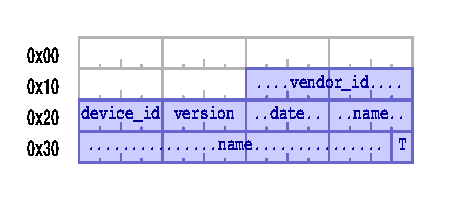
\includegraphics[width=100mm]{img/sdb-product.ps}
\caption{The Product Structure}
\label{fig:FigureProduct}
\end{figure}

\begin{center}
  \begin{savenotes}
    \begin{table}[!ht]\footnotesize
      \caption{SDB Product Structure (40 bytes, at offset 24)}\label{sdb_product}\centering
        \begin{tabular}{| c | c | c | l | c | p{5cm} |} \hline
        First & Last & Size & Name & Value & Description \\ \hline
        0x18 & 0x1f & 8 & vendor\_id & - & 64-bit vendor ID \\ \hline
        0x20 & 0x23 & 4 & device\_id & - & 32-bit vendor specific device ID \\ \hline
        0x24 & 0x27 & 4 & version & - & Vendor specific device version number \\ \hline
        0x28 & 0x2b & 4 & date & - & The release date (hex format, eg. 0x20120621) \\ \hline
        0x2c & 0x3e & 19 & name & - & UTF-8 device name, 0x20 filled, without terminator \\ \hline
        0x3f & 0x3f & 1 & record\_type & - & Record type byte (see Table \ref{record_type}) \\ \hline
        \end{tabular}
    \end{table}
  \end{savenotes}
\end{center}

\begin{description}
\item[vendor\_id] \hfill \\
This field provides a 64 bit field that identifies the vendor of the device. The vendor may
be a company, an organization or an individual. The vendor name space is split in two halves;
anybody \textbf{can} pick a vendor ID in the upper half (first bit set), and the
63 bits \textbf{must} be picked as a random number and \textbf{should} be used consistently
in all designs by this vendor.

A registry is still needed to prevent collisions when using community developed designs from
multiple sources, and one should be set up as you read this.
Entities that want a more official vendor
ID than a random number, \textbf{should} apply with the current registry using a number of their choice.
Small
numbers \textbf{should} be avoided, preferring more meaningful strings instead. The
registry \textbf{should} reject numbers smaller than 12 bits, and \textbf{may} reject numbers
according to policies other than collisions with other vendors.

\item[device\_id] \hfill \\
This field specifies a vendor-defined device ID for the device being described.
Vendors are free to manage these 32 bits as they like, but they \textbf{should} use
the same identifier for fully compatible implementations, using other fields like \textit{version}
and \textit{date} to differentiate them.

\item[version] \hfill \\
This field specifies a vendor-defined version number for the device. Vendors
\textbf{can} use the bits as they wish; for example, this \textbf{may} be used sequentially
or \textbf{may} be derived from the information provided by the source code management in use
for gateware source code.


\item[date] \hfill \\
Design/release date of the product. This \textbf{must} be either 0 (unspecified) or a 32-bit hex
format number in the format 0xYYYYMMDD. For example, 0x20120621.

\item[name] \hfill \\
The UTF-8 name of the device. As long as the name fits in 19 bytes, designers are free to choose
any string (e.g. both ``\texttt{UART}`` or ``\texttt{8250-like Serial}'' are valid names).
The name \textbf{should} be a single word or an hyphenated word, avoiding spaces, because it \textbf{may}
be used by driver software to generate pathnames.  The string \textbf{must} start at offset 0
and \textbf{must} be feature value 0x20 (space) in all trailing bytes.
It \textbf{must not} have a trailing zero byte.

\item[record\_type] \hfill \\
Since the product structure is at the end of the SDB record, it includes the
type field. You can access the field from any SDB record, because all records feature
the type byte at offset 0x3f.  Software \textbf{must} verify this field before trying to
make sense of any other field in the SDB record.
There is a record type for each different
SDB record, and the header file gives it a symbolic name through \texttt{enum}.
The currently defined record types are listed in Table \ref{record_type}.  New
record types will most likely enter this specification over time, without the need
to change the SDB version or overall layout.  Users adding new record types \textbf{must}
choose a yet-unused value with the hight bit clear for \textit{component} records (0-127);
users adding new record types of informative value (a \textit{product} or a completely
different structure) \textbf{must} choose a yet-unused value with the high bit set (128-255).
Local or temporary uses \textbf{should} fall in the ranges 0x70-0x7f and 0xf0-0xfe.
Software \textbf{should} report a warning when if finds an
unknown record type in the range 0x00-0x7f is found; unknown records in the range 0x80-0xff
\textbf{can} be ignored silently.
\end{description}

\begin{center}
  \begin{savenotes}
    \begin{table}[!ht]\footnotesize
      \caption{SDB Record Types}\label{record_type}\centering
        \begin{tabular}{| c | l | p{6cm} |} \hline
        Name & Value & Description \\ \hline
        sdb\_type\_interconnect & 0x00 & Interconnect record, first of a table \\ \hline
        sdb\_type\_device & 0x01 & Device definition \\ \hline
        sdb\_type\_bridge & 0x02 & Bridge to a sub-bus \\ \hline
        & 0x03-0x6f & Reserved for future types \\ \hline
        & 0x70-0x7f & Local/temporary use \\ \hline
        sdb\_type\_integration & 0x80 & Informative: integration structure \\ \hline
        sdb\_type\_repo\_url & 0x81 & Informative: repository location \\ \hline
        sdb\_type\_synthesis & 0x80 & Informative: synthesis details \\ \hline
        & 0x83-0xef & Reserved for future informative records \\ \hline
        & 0xf0-0xfe & Local/temporary use \\ \hline
        sdb\_type\_empty & 0xff & Empty record \\ \hline
        \end{tabular}
    \end{table}
  \end{savenotes}
\end{center}

\pagebreak 

\subsection{SDB Component Structure}

The SDB Component is described by a data structure that includes \textit{product}
information. It provides information regarding the address space used by the
component it describes.

\begin{figure}[h]
\centering%
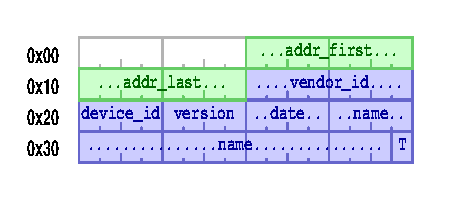
\includegraphics[width=100mm]{img/sdb-component.ps}
\caption{The Component Structure}
\label{fig:FigureComponent}
\end{figure}

\begin{center}
  \begin{savenotes}
    \begin{table}[!ht]\footnotesize
      \caption{SDB Component Structure (56 bytes, at offset 8)}\label{sdb_component}\centering
        \begin{tabular}{| c | c | c | l | c | p{5cm} |} \hline
        First & Last & Size & Name & Value & Description \\ \hline
        0x08 & 0x0f & 8 & addr\_first & - & The first valid address of the component \\ \hline
        0x10 & 0x17 & 8 & addr\_last & - & The last valid address of the component \\ \hline
        0x18 & 0x3f & 40 & product & - & SDB Product structure (see Table \ref{sdb_product} \\ \hline
        \end{tabular}
    \end{table}
  \end{savenotes}
\end{center}

\begin{description}
\item[addr\_first] \hfill \\
The field \textbf{must} represent the first byte address that belongs to this component,
within the encompassing bus. If the address bits in the bus are less than 64, the
unused most significant bits must be cleared. (e.g.: 0x0000.0000.0400.0000)

\item[addr\_last] \hfill \\
The field \textbf{must} represent the last byte address that belongs to this component,
within the encompassing bus. If the address bits in the bus are less than 64, the
unused most significant bits must be cleared. (e.g.: 0x0000.0000.0400.ffff).
This field \textbf{must not} represent the first invalid address (e.g.: 0x0000.0000.0401.0000).

\item[product] \hfill \\
This is the embedded 40 byte product info structure as described in Table \ref{sdb_product}.
\end{description}

\subsection{SDB Records}

This subsection describes the currently defined SDB records that build an SDB array.
These
structures must be instantiated by designers for each logic block in their design and compiled into
a contiguous SDB table, placed at a known address in the bus memory.  Most of these structures
include a \textit{component} structure or a \textit{product} structure, and the rules for the
respective fields apply.

\pagebreak 

\subsubsection{SDB Interconnect}

The \textit{interconnect} record describes the overall bus or bus subset. Every
SDB table \textbf{must} feature such structure as first one in the array.

\begin{figure}[h]
\centering%
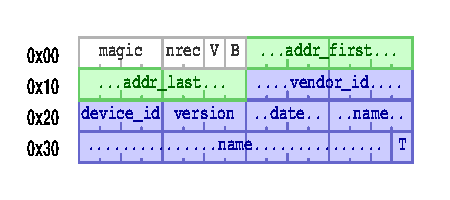
\includegraphics[width=100mm]{img/sdb-interconnect.ps}
\caption{The Interconnect Structure}
\label{fig:FigureInterconnect}
\end{figure}

\begin{center}
  \begin{savenotes}
    \begin{table}[!ht]\footnotesize
      \caption{SDB Interconnect Record (64 bytes, type 0x00)}\label{sdb_interconnect}\centering
        \begin{tabular}{| c | c | c | l | c | p{4cm} |} \hline
        First & Last & Size & Name & Value & Description \\ \hline
        0x00 & 0x03 & 4 & sdb\_magic & 0x5344422D & ``SDB-'', used to verify a table is actually there \\ \hline
        0x04 & 0x05 & 2 & sdb\_records & - & Number of records in this SDB table (including this one) \\ \hline
        0x06 & 0x06 & 1 & sdb\_version & 1 & SDB format version. Currently 1 \\ \hline
        0x07 & 0x07 & 1 & sdb\_bus\_type & - & The bus type for all components in the table \\ \hline
        0x08 & 0x3f & 56 & sdb\_component & - & SDB Component structure (see Table \ref{sdb_component} \\ \hline
        \end{tabular}
    \end{table}
  \end{savenotes}
\end{center}

\begin{description}
\item[sdb\_magic] \hfill \\
The field \textbf{must} be set to 0x5344422D. If you use a similar data structure but
choose to not fully comply to this standard, you \textbf{must} use a different magic
number.
% can people comply with this ``must'' clause, if they choose not to comply with SDB?

\item[sdb\_records] \hfill \\
This field specifies the number of records in the table. It \textbf{must} include
this very record in the count, and the whole address range (this number multiplied by 64 bytes)
\textbf{must} be accessible. Note that the array \textbf{may} include empty records at any position.

\item[sdb\_version] \hfill \\
This is the record format version. In the current version of the specification this is the
value 0x01. If software finds an unknown version number it \textbf{must} abort enumeration.

\item[sdb\_bus\_type] \hfill \\
This field specifies the bus type. This field is used when decoding the bus specific information
inside a device record (see below).  All records in the array share the same
bus type, bus-specific bits in each device declare the details for data access.

Table \ref{bus_type} lists the currently defined types.

\item[sdb\_component] \hfill \\
An interconnect record describes a \textit{component}, so it embeds a component structure.
The \textit{type} field in the component is 0x00.
\end{description}


\begin{center}
  \begin{savenotes}
    \begin{table}[!ht]\footnotesize
      \caption{SDB Bus Types}\label{bus_type}\centering
        \begin{tabular}{| c | l | p{5cm} |} \hline
        Name & Value & Description \\ \hline
        WishBone & 0x00 & Specifies a Wishbone bus type, as commonly used in FPGAs \\ \hline
        Storage & 0x01 & Specifies use of SDB records as a simple filesystem \\ \hline
        \end{tabular}
    \end{table}
  \end{savenotes}
\end{center}


\pagebreak 

\subsubsection{Device Record}

This record type describes a single device or logic block mapped into the memory of the
bus. In a compliant implementation, one device record \textbf{should} exist for each device that is
connected to the bus. Users \textbf{may} choose to aggregate a complex device under a single
description record. The structure of the device record is shown below in Table
\ref{sdb_device}.

\begin{figure}[h]
\centering%
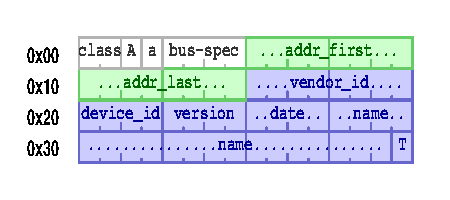
\includegraphics[width=100mm]{img/sdb-device.ps}
\caption{The Device Structure}
\label{fig:FigureDevice}
\end{figure}

\begin{center}
  \begin{savenotes}
    \begin{table}[!ht]\footnotesize
      \caption{SDB Device Record (64 bytes, type 0x01)}\label{sdb_device}\centering
        \begin{tabular}{| c | c | c | l | c | p{5cm} |} \hline
        First & Last & Size & Name & Value & Description \\ \hline
        0x00 & 0x01 & 2 & abi\_class & - & The ABI class of the device (0 = Custom Device) \\ \hline
        0x02 & 0x02 & 1 & abi\_ver\_major & - & The ABI major version \\ \hline
        0x03 & 0x03 & 1 & abi\_ver\_minor & - & The ABI minor version \\ \hline
        0x04 & 0x07 & 4 & bus\_specific & - & Bus specific field (flags) \\ \hline
        0x08 & 0x3f & 56 & sdb\_component & - & SDB Component Info structure \\ \hline
        \end{tabular}
    \end{table}
  \end{savenotes}
\end{center}

\begin{description}
\item[abi\_class] \hfill \\
The ABI class, if not 0, tells the kind of standard interface that the device provides. This
allows a single driver to deal with compatible devices designed by different vendors, not unlikely
PCI or USB classes.  Currently, no ABI class is defined. Designers \textbf{should} use 0 here,
until an official SDB class registry exists.

\item[abi\_ver\_major] \hfill \\
This is the major version number of the ABI class. Standard interfaces are not compatible between
major version changes.  If the class is 0, designers \textbf{can} use this field of driver-specific uses. For
example, a driver can be able to deal with a number of similar devices (all with a different device-ID)
and use the ABI fields as a hint to classify the various devices.

\item[abi\_ver\_minor] \hfill \\
This is the minor version number of the ABI class. Standard interfaces are compatible between
minor version changes. Again, if the class is 0, developers \textbf{can} set this field for internal use.

\item[bus\_specific] \hfill \\
This is a 4-byte field that holds bus-specific information, most likely flags. For current
values, please refer to header files.

\item[component] \hfill \\
This is a standard \textit{component} structure (see Table \ref{sdb_component}). The record type
for a device is 0x01.
\end{description}

\pagebreak 

\subsubsection{Bridge Record}

A bridge record is used to describe a nested bus within the same address space.  Bus
structures with nested interconnects are typical in complex projects.
The structure of the bridge record is shown in Table \ref{sdb_bridge}.

\begin{figure}[h]
\centering%
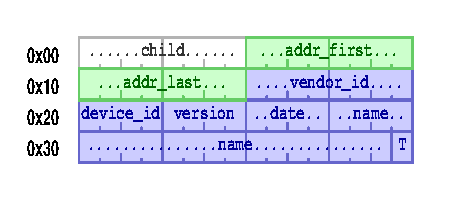
\includegraphics[width=100mm]{img/sdb-bridge.ps}
\caption{The Bridge Structure}
\label{fig:FigureBridge}
\end{figure}

\begin{center}
  \begin{savenotes}
    \begin{table}[!ht]\footnotesize
      \caption{SDB Device Record (64 bytes, type 0x02)}\label{sdb_bridge}\centering
        \begin{tabular}{| c | c | c | l | c | p{5cm} |} \hline
        First & Last & Size & Name & Value & Description \\ \hline
        0x00 & 0x07 & 8 & sdb\_child & - & The relative address of the nested SDB table \\ \hline
        0x08 & 0x3f & 56 & sdb\_component & - & SDB Component structure \\ \hline
        \end{tabular}
    \end{table}
  \end{savenotes}
\end{center}

\begin{description}
\item[sdb\_child] \hfill \\
This field gives the location of the nested bus' SDB table. This address is a relative address
with respect to the start of the this address space -- not the nested one. In other words,
all addresses in this SDB array are relative to the same base address; this ensures consistency
within each SDB array and allows the ROM area that describes a sub-interconnect to be
outside the interconnect itself.  Designers can thus describe the internals of legacy logic
cores without the need to change them.
The value \textbf{must} point to an SDB array that begins with an \textit{interconnect} record.
\textbf{Note}: version 1.0 of the specification
got this point wrong, contrary to all existent implementations.

\item[component] \hfill \\
An embedded component info structure, where the type is 0x01 See Table \ref{sdb_component}.
\end{description}

\pagebreak 

\subsubsection{Integration Record}

An integration record is a \textit{product} record (not a \textit{component}, because
it has no associated address range).
The structure provides meta-data about the aggregate product of the bus or bus subset.
For example, consider
a manufacturer that takes components from various vendors and combines them with a standard bus
interconnect. This aggregate product can be described by an SDB integration record, claiming
a vendor ID, the release date and the other \textit{product} information.
The integration record is is described in Table \ref{sdb_integrator}.

\begin{figure}[h]
\centering%
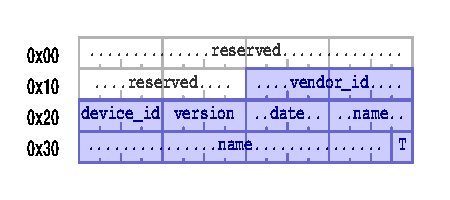
\includegraphics[width=100mm]{img/sdb-integration.ps}
\caption{The Integration Structure}
\label{fig:FigureIntegration}
\end{figure}

\begin{center}
  \begin{savenotes}
    \begin{table}[!ht]\footnotesize
      \caption{SDB Integrator Record (64 bytes, type 0x80)}\label{sdb_integrator}\centering
        \begin{tabular}{| c | c | c | l | c | p{5cm} |} \hline
        First & Last & Size & Name & Value & Description \\ \hline
        0x00 & 0x1f & 24 & reserved & - & Reserved/unused space \\ \hline
        0x18 & 0x3f & 40 & product & - & SDB Product Info structure \\ \hline
        \end{tabular}
    \end{table}
  \end{savenotes}
\end{center}

\begin{description}
\item[reserved] \hfill \\
The initial field in this record is unused, because all needed information is
part of the product structure. Users \textbf{should} fill this area with all bits
clear or all bit set.

\item[product] \hfill \\
This is the \textit{product} structure described in Table \ref{sdb_product}. The
record type for an integration record is 0x80.
\end{description}

\pagebreak 

\subsubsection{Repository-Url Record}

This record is not a \textit{product}; it is laid out as a simple 63-byte string
that reports the URL of the repository used to driver this synthesis.
This record is optional like all other informational structures, but we think it's
useful for designers to have a standardized way to allow tracing the design.
Actually, this data structure is already implemented in one ADC design.

\begin{figure}[h]
\centering%
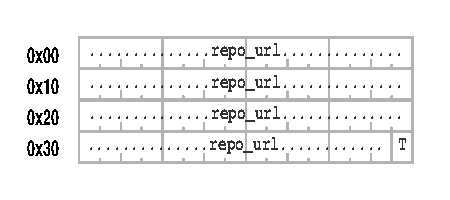
\includegraphics[width=100mm]{img/sdb-url.ps}
\caption{The Repository-Url Structure}
\label{fig:FigureUrl}
\end{figure}

\begin{center}
  \begin{savenotes}
    \begin{table}[!ht]\footnotesize
      \caption{SDB Repository-Url Record (64 bytes, type 0x81)}\label{sdb_url}\centering
        \begin{tabular}{| c | c | c | l | c | p{5cm} |} \hline
        First & Last & Size & Name & Value & Description \\ \hline
        0x00 & 0x3e & 63 & repo\_url & - & Repository for this design \\ \hline
        0x3f & 0x3f & 1 & record\_type & 0x81 & Type of this record \\ \hline
        \end{tabular}
    \end{table}
  \end{savenotes}
\end{center}

\begin{description}
\item[repo\_url] \hfill \\
This is a string, encoded in  UTF-8, with trailing spaces and no terminating 0.
It is expected to name the top-level repository
used to build this design, as a \texttt{git://} or \texttt{http://} form or
anything appropriate for the revision control system being used.

\item[record\_type] \hfill \\
The record type for this structures is 0x81.
\end{description}

\pagebreak 

\subsubsection{Synthesis Record}

This record, like the previous one, is not a \textit{product}.
The record is optional, but it reveals
useful to stanrdadize the way to provide information about the specific synthesis.
Not all designers want to provide such detailed information, but when they
do they  \textbf{should} use this format.

Please note that the information in this record is pretty volatile, as
it represents the actual synthesis; if the record is used, developers
must be careful to update (or remove) it when they rebuild the
project.  All unused fields can be left empty, but all non-empty fields should be updated
with great care or the initial effort to provided detailed tracking is voided.

\begin{figure}[h]
\centering%
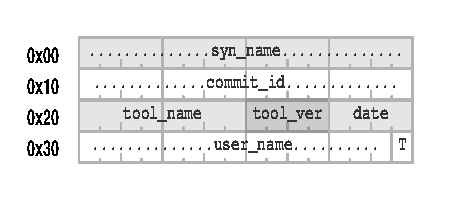
\includegraphics[width=100mm]{img/sdb-synthesis.ps}
\caption{The Synthesis Structure}
\label{fig:FigureSynthesis}
\end{figure}

\begin{center}
  \begin{savenotes}
    \begin{table}[!ht]\footnotesize
      \caption{SDB Synthesis Record (64 bytes, type 0x82)}\label{sdb_synthesis}\centering
        \begin{tabular}{| c | c | c | l | c | p{5cm} |} \hline
        First & Last & Size & Name & Value & Description \\ \hline
        0x00 & 0x0f & 16 & syn\_name & - & Name of this project/synthesis \\ \hline
        0x10 & 0x1f & 16 & commit\_id & - & Identifier of the build commit \\ \hline
        0x20 & 0x27 & 8 & tool\_name & - & Name of the synthesis tool \\ \hline
        0x28 & 0x2b & 4 & tool\_version & - & Version of the synthesis tool \\ \hline
        0x2c & 0x2f & 4 & date & - & Date of synthesis \\ \hline
        0x30 & 0x3e & 15 & user\_name & - & Name of the user who did the synthesis \\ \hline
        0x3f & 0x3f & 1 & record\_type & 0x82 & Type of this record \\ \hline
        \end{tabular}
    \end{table}
  \end{savenotes}
\end{center}

\begin{description}
\item[syn\_name] \hfill \\
This is a string, encoded in  UTF-8, with trailing spaces and no terminating 0;
it should represent a human-readable name for this synthesis. Like all other
fields in this structures, it is meant to be useful for the designers, to help
tracking what is currently installed in the various systems.  Thus, this may
be a generic name of the project or a more specific string, according to local
needs.

\item[commit\_id] \hfill \\
This field represents the binary identifier of the top-level commit used
to build this gateware image. If the identifier is more than 128 bits long
(e.g., \textit{git}), the field includes the leading bits. If the commit ID is numeric
(e.g., SVN), the representation is bit-endian binary. For repositories using
non-binary version numbers, the representation is let to the ingenuity of the
developer, to properly convey the informations. For example, a CVS version
like ``1.20.1.4'' can either be ASCII-encoded or represented as 4 32-bit big-endian
fields.  Clearly, the commit\_id field raises a ``chicken-and-egg'' problem: once
you commit the change, your commit identifier changes, maybe in unpredictable
ways. Representing the ``previous'' commit, and then committing and sdb-only
change is a sensible workaround.  The filed \textbf{should} be 0 if not used.


\item[tool\_name] \hfill \\
This is a string, encoded in  UTF-8, with trailing spaces and no terminating 0;
it represents a human-readable name for the synthesis tool used to build this
very binary gateware file.

\item[tool\_version] \hfill \\
The version of the synthesis tool, in a human-readable way. For example,
it can be used as two 16-bit fields, but this really depends on how the specific
tool names its versions.

\item[date] \hfill \\
The date of synthesis.  This \textbf{must} be either 0 (unspecified) or a 32-bit hex
format number in the format 0xYYYYMMDD. For example, 0x20130327.

\item[user\_name] \hfill \\
This is a string, encoded in  UTF-8, with trailing spaces and no terminating 0;
it states who is the user who built the binary gateware.  This name is expected
to be unique among the development group, so a Unix username or a nickname are good
choices that fit the allowed space of 15 bytes.

\item[record\_type] \hfill \\
The record type for this structures is 0x82.
\end{description}

\pagebreak 

\section{Simple Real-World Examples}

This section shows the details of the simplest real-world example of an SDB array,
and an overlook of a more structured device.

\subsection{Simple Binary Data}

The FPGA binary used as the simplest example is the \textit{boot} image to be
programmed in the SPEC cards
(\texttt{http://www.ohwr.org/projects/spec}); it only includes the
\textit{syscon} device, which allows generic access to the FMC
mezzanine card.

The following binary dump appears at offset 0x100 of the memory window
that maps to the programmable device:

\footnotesize
\begin{verbatim}
000000 53 44 42 2d 00 02 01 00 00 00 00 00 00 00 00 00  >SDB-............<
000010 00 00 00 00 00 00 01 ff 00 00 00 00 00 00 06 51  >...............Q<
000020 e6 a5 42 c9 00 00 00 02 20 12 05 11 57 42 34 2d  >..B..... ...WB4-<
000030 43 72 6f 73 73 62 61 72 2d 47 53 49 20 20 20 00  >Crossbar-GSI   .<
000040 00 00 01 01 00 00 00 07 00 00 00 00 00 00 00 00  >................<
000050 00 00 00 00 00 00 00 ff 00 00 00 00 00 00 ce 42  >...............B<
000060 ff 07 fc 47 00 00 00 01 20 12 03 05 57 52 2d 50  >...G.... ...WR-P<
000070 65 72 69 70 68 2d 53 79 73 63 6f 6e 20 20 20 01  >eriph-Syscon   .<
\end{verbatim}
\normalsize

\subsection{Parsing the Data}

This is the suggested parsing sequence for the data shown above. The
parsing code is assumed to know where the data structure is expected to live.

\begin{itemize}
\item The parser verifies the magic number 0x5344422D at offset 0.
\item The type byte of 0x00 at offset 0x3f confirms this is an \textit{interconnect} record.
\item The SDB version, at offset 6, confirms this is version 1 and we can parse it.
\item By reading the 16-bit field at position 04-05, we know this is an array of two items.
\item The second item is of type \textit{device} (type 0x01).
\end{itemize}

What follows is the split-out view of the two structures:

\footnotesize
\begin{verbatim}
Interconnect:
0x00:   53 44 42 2d               (Magic "SDB-")
0x04:   00 02                     (Number of records)
0x06:   01                        (SDB version)
0x07:   00                        (Bus type: wishbone)
0x08:   00 00 00 00 00 00 00 00   (First address)
0x10:   00 00 00 00 00 00 01 ff   (Last address)
0x18:   00 00 00 00 00 00 06 51   (Vendor: GSI)
0x20:   e6 a5 42 c9               (Device)
0x24:   00 00 00 02               (Version)
0x28:   20 12 05 11               (Date: 11th May 2012)
0x2c:   "WB4-Crossbar-GSI   "     (Name)
0x3f:   00                        (Type: interconnect)

Device:
0x00:   00 00                     (ABI class)
0x02:   01                        (ABI version major)
0x03:   01                        (ABI version minor)
0x04:   00 00 00 07               (Bus-specific: BE, 8,16,32 bits)
0x08:   00 00 00 00 00 00 00 00   (First address)
0x10:   00 00 00 00 00 00 00 ff   (Last address)
0x18:   00 00 00 00 00 00 ce 42   (Vendor: CERN)
0x20:   ff 07 fc 47               (Device)
0x24:   00 00 00 01               (Version)
0x28:   20 12 03 05               (Date: 5th March 2012)
0x2c:   "WR-Periph-Syscon   "     (Name)
0x3f:   01                        (Type: device)
\end{verbatim}
\normalsize

The previous dump shows how the vendor identifiers in this case have
been allocated in the globally-assigned space, while device identifiers
are pseudo-random numbers, in charge of the respective vendor.

\subsection{A More Structured Device}

The following is the output of \texttt{eb-ls}, and \textit{Etherbone}
tool, when run over a complex White Rabbit device. This output
comes from scanning the SDB structures:

\footnotesize
\begin{verbatim}
root@scul007:~# eb-ls dev/pcie_wb0
BusPath   VendorID         Product   Base(Hex)  Description
1         000000000000ce42:66cfeb52         0  WB4-BlockRAM
2         0000000000000651:eef0b198    100000  WB4-Bridge-GSI
2.1       0000000000000651:35aa6b95    100000  GSI_GPIO_32
2.2       0000000000000651:8752bf44    140000  GSI_ECA_UNIT
2.3       0000000000000651:10051981    180000  GSI_TM_LATCH
3         0000000000000651:eef0b198    200000  WB4-Bridge-GSI
3.1       000000000000ce42:66cfeb52    200000  WB4-BlockRAM
3.2       0000000000000651:eef0b198    220000  WB4-Bridge-GSI
3.2.1     000000000000ce42:ab28633a    220000  WR-Mini-NIC
3.2.2     000000000000ce42:650c2d4f    220100  WR-Endpoint
3.2.3     000000000000ce42:65158dc0    220200  WR-Soft-PLL
3.2.4     000000000000ce42:de0d8ced    220300  WR-PPS-Generator
3.2.5     000000000000ce42:ff07fc47    220400  WR-Periph-Syscon
3.2.6     000000000000ce42:e2d13d04    220500  WR-Periph-UART
3.2.7     000000000000ce42:779c5443    220600  WR-Periph-1Wire
3.2.8     000000000000ce42:779c5443    220700  WR-Periph-1Wire
\end{verbatim}
\normalsize

\subsection{Endianness Problems}

Please note that the host may have some issues reading the binary
dumps. According to how the bridge between the host and FPGA is
designed you may face one of the following situations:

\begin{itemize}
\item The host is big-endian (data is always correct).
\item The host is little-endian and the bridge is byte-oriented.
\item The host is little-endian and the bridge is word-oriented.
\end{itemize}

If the bridge is byte-oriented, i.e. each and every byte can be
independently addressed as such, then the usual endian conversion
rules apply (e.g. you can \textit{memcpy} the records to host memory
and access fields with endian-aware code).

If the bridge is word-oriented, with 32-bit words in this example, the behaviour is stranger, in
a way.  After you copied the data to host memory (whether one byte at
a time or not), you'll find that the bytes are swapped within each word.
This happens because the 32-bit word is transferred as a whole: the least significant
bits remain the the least significant, but they come from offset 3 in the data structure
and are stored at offset 0 in the little-endian host.  If this is your case, you need to
byte-swap each 32-bit word before using the structure in a
little-endian host. After such swapping, the data fields live at the correct
offsets and must be accessed as big endian.

\subsection{References}

The \textit{Etherbone} project, is an early adopter of SDB;
it includes also a number
of tools that work with SDB structures (including \texttt{eb-ls} that
printed the table of devices shown above).  The project is at
\texttt{http://www.ohwr.org/projects/etherbone-core} .

The \textit{sdbfs} work started as a separate project but it is now
part of the \texttt{fpga-config-space} project.  It is currently work
in progress, but the \textit{gensdbfs} and other non-kernel parts are already
being used in production.

\end{document}

% LocalWords:  metadata FPGA gateware CERN endian etherbone filesystem
